\documentclass[14pt]{beamer}
\usepackage[latin1]{inputenc}
\usepackage{graphics}
\usepackage{hyperref}
\usetheme{Warsaw}
\setbeamertemplate{navigation symbols}{}
\title{The Basics of Git}
\begin{document}
\begin{frame}
\titlepage
\end{frame}

\begin{frame}{What is Git?}
	According to the documentation:\newline
	"git" can mean anything, depending on your mood.
	\begin{itemize}
		\small
		\item random three-letter combination that is pronounceable, and not
		   actually used by any common UNIX command.  The fact that it is a
		   mispronunciation of "get" may or may not be relevant.
		\item stupid. contemptible and despicable. simple. Take your pick from the
		   dictionary of slang.
		\item "global information tracker": you're in a good mood, and it actually
		   works for you. Angels sing, and a light suddenly fills the room.
		\item "godd*mn idiotic truckload of sh*t": when it breaks
	\end{itemize}
\end{frame}

\begin{frame}{What is Git?}
	Git is a fast, scalable, distributed revision control system with an
	unusually rich command set that provides both high-level operations
	and full access to internals.
\end{frame}

\begin{frame}{What is Git?}
	\begin{itemize}
		\item Git is flexible for many different workflows.
		\item Git is non-linear.
		\item Git stores all data locally and is therefore much faster.
		\item Git is distributed.  This means it allows for many
			developers to work independenty, yet collaboratively.
		\item Git allows a deveoper to seamlessly switch between features(branches).
		\item Git allows for disposable experimentation.
	\end{itemize}
\end{frame}


\begin{frame}{Getting started}
	\begin{enumerate}
		\small
		\item Install git. (mSysGit on Windows)\newline
		\href{http://msysgit.googlecode.com/files/Git-1.7.11-preview20120710.exe}{http://msysgit.googlecode.com/files/Git...}
		\href{http://goo.gl/uXDLa}{http://goo.gl/uXDLa}
		\item Get a github account
		\item Set up SSH keys
		\item Forking a repository\newline
		\href{https://github.com/guywithnose/Git-training}{https://github.com/guywithnose/Git-training}
		\href{http://goo.gl/EDor7}{http://goo.gl/EDor7}
		\item Clone your fork
		\item Commit
		\item Push
		\item Merge/Pull Request
	\end{enumerate}
\end{frame}


\begin{frame}{Basic commands}
	\begin{itemize}
		\item add
		\item reset
		\item status
		\item commit
		\item log
		\item diff
		\item show
	\end{itemize}
\end{frame}

\begin{frame}{Staging area}
	\begin{figure}[htb]
		\centering
		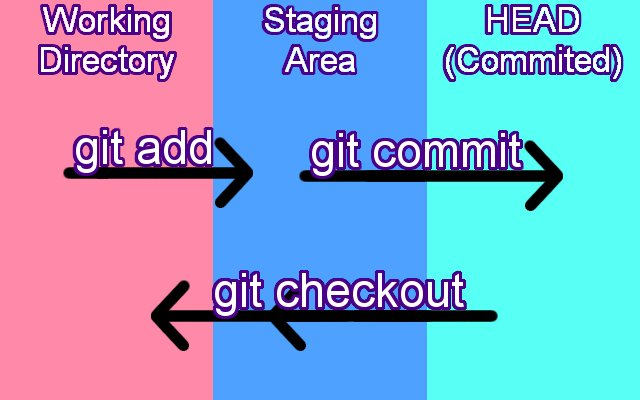
\includegraphics[width=\textwidth]{commit-add-reset.jpg}
	\end{figure}
\end{frame}

\begin{frame}{What is a commit}
	You can see this with cat-file
	\begin{figure}[htb]
		\centering
		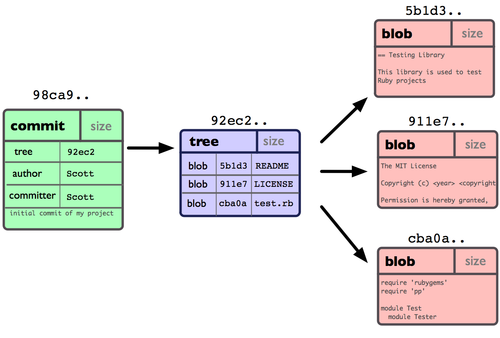
\includegraphics[width=\textwidth]{commitBlobs.png}
	\end{figure}
\end{frame}

\begin{frame}{What is a commit}
	\begin{figure}[htb]
		\centering
		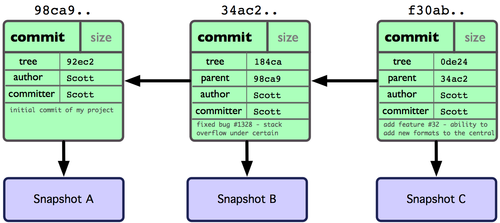
\includegraphics[width=\textwidth]{commitSnapshots.png}
	\end{figure}
\end{frame}

\begin{frame}{Git is non linear}
	Unlike SVN git is not linear.  A commit can have two parents.  It can also have many children... Kinda like people.
	\begin{figure}[htb]
		\centering
		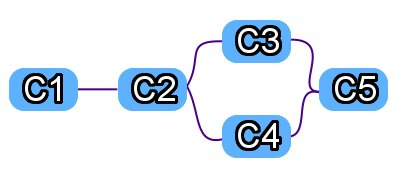
\includegraphics[width=\textwidth]{nonLinearCommits.jpg}
	\end{figure}
\end{frame}

\begin{frame}{How do we use branches?}
	\begin{figure}[htb]
		\centering
		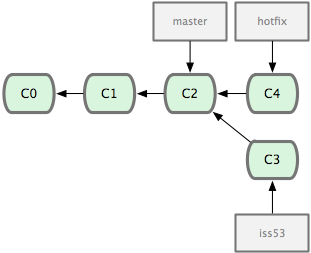
\includegraphics[width=.7\textwidth]{hotfix.png}
	\end{figure}
\end{frame}

\begin{frame}{How do we use branches?}
	\begin{figure}[htb]
		\centering
		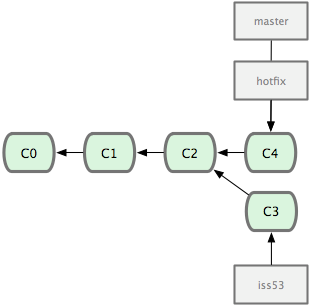
\includegraphics[width=.7\textwidth]{hotfix2.png}
	\end{figure}
\end{frame}

\end{document}